\todo{section intro}

\subsection{Genetic algorithms}

A genetic algorithm (GA) is a very common type of EA.
It represents each solution as a genotype, a binary string describing how the solution itself, the phenotype, should be constructed.
The genotype is comparable to nature's DNA, and it is this genetic material which is modified in the evolutionary process.

\begin{figure}[!ht]
    \centering
    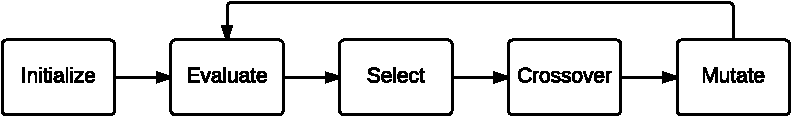
\includegraphics[width=0.48\textwidth]{figures/ga}
    \caption{A genetic algorithm. The cycle is broken when the fitness is above a given threshold.}
    \label{fig:ga}
\end{figure}

The GA process is shown in \figurename~\ref{fig:ga}.
First, a base population with random genotypes is constructed.
Then, each phenotype is constructed and evaluated using a fitness function.
If a solution has a fitness score above a set threshold, the process stops.
Otherwise, a new population is created by selecting solutions with high fitness scores, crossing their genotypes, and mutating the results.
Then the process repeats.

\subsection{Development}

The process that transforms the genotype into a phenotype is called development.
It can be regarded as a form of decompression algorithm \cite{harding2008artificial}.
In nature, this process is seen when a fertilized egg transforms into a multicellular organism.
An example is shown in \figurename~\ref{fig:development}.

\begin{figure}[!ht]
    \centering
    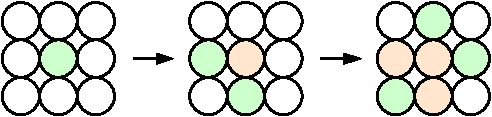
\includegraphics[width=0.30\textwidth]{figures/development}
    \caption{An example of one cell developing into six. Additionally, some cells change type.}
    \label{fig:development}
\end{figure}

Development also allows individuals to adapt to their environments, making them more robust and scalable \cite{tufte2008evodevo}.

\subsection{Cellular automata}

\todo{resembles biological stuff}

A cellular automaton (CA) is a structure made up of vast numbers of very simple computational units called cells.
The cells are arranged in a grid, with communication only permitted between nearby cells according to a neighborhood.
The von Neumann neighborhood is common for two-dimensional CAs \CN;
It includes the cells to the north, south, east and west, along with itself (center).
An example of this is shown in \figurename~\ref{fig:ca}.

\begin{figure}[!ht]
    \centering
    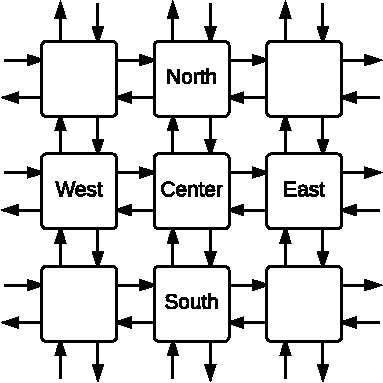
\includegraphics[width=0.25\textwidth]{figures/ca}
    \caption{An excerpt from a 2D CA using a von Neumann neighborhood. All outputs from a given cell carries the same value.}
    \label{fig:ca}
\end{figure}

Each cell has a state, which is often a binary number where 1 represents alive and 0 represents dead.
At each discrete time step, each cell updates its state based on the states in its neighborhood.
The update function is often specified as a look-up-table (LUT), where the next state is defined for all possible neighborhood states\footnotemark.
\footnotetext{
    The length of the LUT increases exponentially with the size of the neighborhood.
    $L=S^N$ where $L$ is the LUT length, $S$ is the number of possible states and $N$ is the number of cells in the neighborhood.
}
If all cells implement the same update function then the CA is uniform, otherwise it is non-uniform.

CAs have been shown to be Turing complete \cite{neumann1966selfreplication} \cite{codd1968cellular}, which means they are able to perform any kind of computation.

\todo{expand}
Usage in EHW:
Langton's research on emergent computation and phase transition \cite{langton1990edgeofchaos}.
Wolfram's four qualitative CA classes \cite{wolfram1984complexity}.

Due to their resemblance to biological systems, CAs have been 

Self-Replication:
von Neumann's work on self-replication from around 1950 \cite{neumann1966selfreplication}.
Self-replicating structures \cite{reggia1998neumann}.
Replicating universal computers with 63 states and 8500 rules \cite{perrier1996toward}.
\todo{/expand}

\subsection{Field Programmable Gate Array}

A Field Programmable Gate Array (FPGA) is a type of reconfigurable hardware.
It can implement any desired logical operation by configuring and connecting a number of look-up tables (LUTs) and flip-flops (FFs).
FPGAs can also contain dedicated blocks for adding, multiplying, random access memory (RAM) and other functions.
Configurable elements are grouped into configurable logic blocks (CLBs), which through a network of interconnects can be connected to each other or input/output pins.
An example of this structure is shown in \figurename~\ref{fig:fpga}.
Note that modern FPGAs consists of thousands of CLBs and hundreds of I/O pins \cite{ds160}.

\begin{figure}[!ht]
    \centering
    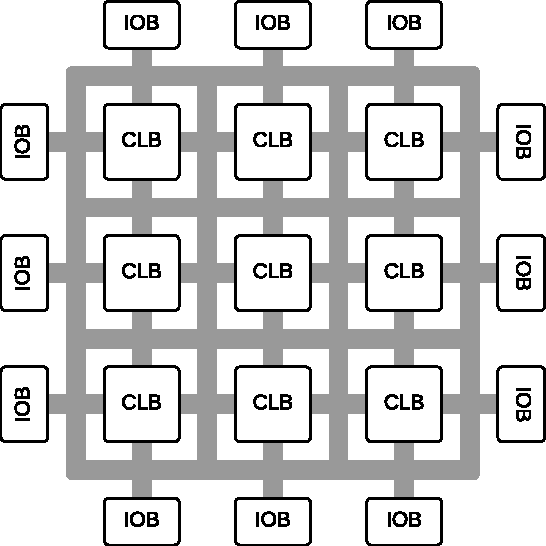
\includegraphics[width=0.30\textwidth]{figures/fpga}
    \caption{High-level block diagram of an FPGA. An array of configurable logic blocks (CLBs) and input/output blocks (IOBs) are connected by a network of interconnects.}
    \label{fig:fpga}
\end{figure}

FPGAs have been the subject of EHW research due to their reconfigurability, and several researchers have been successful in evolving working electronic circuits \cite{huelsbergen1998evolution} \cite{thompson1997evolved}.
However, the resulting circuits have often ended up using intrinsic properties of the silicon and been very sensitive to environmental changes.

The trouble with using modern FPGAs for EHW research is that some configuration bitstrings can destroy the FPGA \cite{ug380} \cite{xapp151}.
This means that the bitstring can not be used directly as the genotype without complicated tests to discard the dangerous bitstrings.

\subsection{Sblock}

The sblock was introduced as part of a new EHW-friendly FPGA architecture in \cite{haddow2000sblock}.
The architecture is a non-uniform CA with a von Neumann neighborhood, where the update function of each cell is independantly configurable at run-time.
Each cell, called an sblock, is a very simple structure; it consists of a configurable look-up-table (LUT) and a flip-flop (FF), as shown in \figurename~\ref{fig:sblock}.

\begin{figure}[!ht]
    \centering
    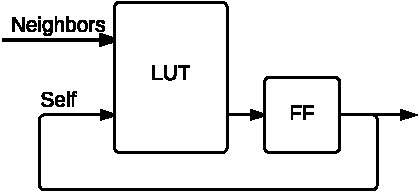
\includegraphics[width=0.25\textwidth]{figures/sblock}
    \caption{Detailed block diagram of an sblock. The LUT can be reconfigured on-the-fly to implement any logical function.}
    \label{fig:sblock}
\end{figure}

The greatest benefit of using sblocks for EHW research is that there is no risk of damage or exploitation of intrinsic properties in the silicon.
Additionaly, the simple structure and hardwired signal routing allows for more efficient area usage than a traditional FPGA.
The likelihood of a mass-produced sblock-FPGA arriving on the market in the near future is slim.
However, it is possible to implement it virtually within another FPGA.

\subsection{PCI Express}

The PCI Express interface was designed to tackle the arising trouble with clocked parallel buses like PCI.
The problem with such buses is that the clock speed can not be increased beyond a given threshold, as the slightly different lengths of the many wires causes data to arrive at slightly different times.
Reducing the clock period to less than the variation in arrival time means the data will become corrupted.
This problem is exacerbated with increasing bus size.

PCI Express is therefore based on serial communication over differential pairs (lanes\footnotemark) without the need for a reference clock \cite{pcie}.
\footnotetext{
    PCI Express operates in full duplex mode, which means that each lane has an independent differential pair in each direction.
    1, 2, 4, 8, 16 or 32 lanes are supported, but data is striped and thus still transmitted serially.
}
This allows an extremely fast clock speed compared to a parallel bus, and much greater bandwidth in total.
PCI Express consists of three layers; the physical layer, the data link layer and the transaction layer, structured as shown in \figurename~\ref{fig:pcie}.

\begin{figure}[!ht]
    \centering
    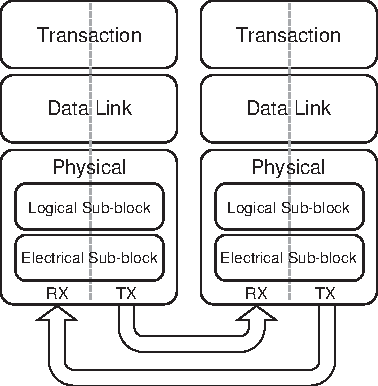
\includegraphics[width=0.25\textwidth]{figures/pcie}
    \caption{High-level diagram showing the layered structure of PCI Express. (Reprinted from \cite{pcie})}
    \label{fig:pcie}
\end{figure}

The transaction layers primary responsibility is the creation and parsing of transaction layer packets (TLPs).
TLPs are used to trigger events or start various transactions, most commonly to initiate read and write requests\footnotemark.
\footnotetext{
    Read and write requests are directed at one of up to six base address registers (BARs).
    They represent internal memory areas that can be anywhere from a few bytes to several gigabytes in size.
}
Most requests entail the return of a completion TLP containing the requested data or other information.
TLPs consists of multiple 32-bit double words (DW), where the first is a common header describing the type of packet.

The data link layer ensures integrity by adding error detection codes to outgoing TLPs and performing error detection and correction on incoming TLPs.
It is also responsible for retransmission if corruption occurs.

The physical layer is responsible for serialization and deserialization of the data stream.
Each byte is padded with two extra bits (8b/10b encoding) to allow clock recovery.

